\documentclass[conference]{IEEEtran}
\IEEEoverridecommandlockouts
\usepackage{cite}
\usepackage{amsmath,amssymb,amsfonts}
\usepackage{algorithmic}
\usepackage{graphicx}
\usepackage{textcomp}
\usepackage{xcolor}
\usepackage{url}
\usepackage{hyperref}
\usepackage{float}
\def\BibTeX{{\rm B\kern-.05em{\sc i\kern-.025em b}\kern-.08em
    T\kern-.1667em\lower.7ex\hbox{E}\kern-.125emX}}

\begin{document}

\title{Analyzing Global Job Market Trends and Skill Demands Using Big Data: A LinkedIn Jobs \& Skills 2024 Study}

\author{
\IEEEauthorblockN{Sahitya Gantala}
\IEEEauthorblockA{\textit{Department of Computer Science} \\
\textit{State University of New York at Buffalo}\\
Buffalo, USA \\
sahityag@buffalo.edu}
\and
\IEEEauthorblockN{Shilpa Ghosh}
\IEEEauthorblockA{\textit{Department of Computer Science} \\
\textit{State University of New York at Buffalo}\\
Buffalo, USA \\
}
\and
\IEEEauthorblockN{Aditya Rajesh Sawant}
\IEEEauthorblockA{\textit{Department of Computer Science} \\
\textit{State University of New York at Buffalo}\\
Buffalo, USA \\
}
}

\maketitle


\begin{abstract}
The LinkedIn Jobs and Skills (2024) dataset, consisting of approximately 1.3 million job postings, provides valuable insights into the global job market by capturing skill requirements, job types, and industry trends. This study implements an end-to-end big data analysis workflow using Hadoop for distributed processing and Pandas for exploratory data analysis (EDA). Our research identifies the most in-demand technical and soft skills, investigates relationships between job types and skill breadth, and discovers regional patterns in workforce specialization. Machine learning techniques are applied for clustering job roles and analyzing skill similarities. The findings highlight key global hiring trends, emphasizing the increasing demand for hybrid skill sets that combine technical proficiency with soft skills such as communication and leadership.
\end{abstract}

\begin{IEEEkeywords}
LinkedIn, Big Data, Hadoop, Skills Analysis, Job Market, Machine Learning
\end{IEEEkeywords}

\section{Introduction}
Over the past decade, Linked-In has become the most influential due to its ability to consolidate comprehensive job related information roles, skills, industries, companies, and career trajectories onto a single digital platform. Unlike traditional job portals, Linked-In integrates professional identity, social connections, and real time labor market data, making it an invaluable source for studying global employment trends and emerging skill demands. 

This unique combination of scale, structure, and context positions Linked-In as an ideal foundation for big data driven workforce analytics.

In this project, we leverage the 1.3 million records of Linked-In Jobs and Skills (2024) dataset to analyze global labor patterns through scalable big data techniques. The dataset encapsulates detailed job attributes such as titles, companies, skills, and employment types, providing a holistic view of the evolving professional landscape. Our study aims to translate this information into actionable insights by implementing a Hadoop-based data pipeline and defining machine learning tasks that uncover trends in skill demand, job clustering, and regional specialization.

The work presented here is aligned with six primary analytical objectives. By combining distributed computing through Hadoop with detailed exploratory and machine learning analysis, this study not only demonstrates scalable data processing but also provides evidence-driven insights into how global labor markets are adapting to digital transformation.


\section{Dataset Description and Cleaning}
The dataset used in this study was obtained from Kaggle’s “1.3M Linked-In Jobs and Skills (2024)” repository, which compiles over 1.3 million Linked-In job postings across multiple industries and countries. The data is organized into three relational tables \textit{job\_postings}, \textit{job\_skills}, and \textit{job\_summary} linked by a common key, \textit{job\_link}. Each table provides complementary information necessary for a comprehensive view of job roles, associated skills, and textual descriptions.

The \textbf{job\_postings} table serves as the primary dataset, containing core job-related information such as job titles, company names, job locations, employment types, seniority levels, and geographic metadata (city and country). It provides the structural foundation for linking with other tables and enables aggregation of postings by region or job type.

The \textbf{job\_skills} table focuses on skill-related attributes, listing both technical and soft skills extracted from each job posting. This table plays a central role in identifying high-demand competencies, analyzing skill co-occurrence, and performing clustering based on skill similarity. Some records were missing skill data, which were flagged or removed depending on analysis needs.

The \textbf{job\_summary} table contains descriptive text from job listings, including roles, responsibilities, and qualification details. These summaries can be used for text mining, natural language processing, or feature extraction tasks that support deeper analysis of job content.

Because the dataset was web-scraped, it exhibited common inconsistencies such as duplicate entries, incomplete fields, and irregular geographic naming conventions. Data cleaning included removing duplicates, standardizing text to lowercase, stripping punctuation, and unifying country representations (e.g., “US,” “U.S.A,” and “United States”). The skills field was tokenized to enable frequency and co-occurrence analysis.


\section{Exploratory Data Analysis (EDA)}
Exploratory Data Analysis (EDA) was conducted to understand the structure and underlying patterns within the LinkedIn Jobs dataset after cleaning and preprocessing. The unified dataset (\textit{final\_df}) combined key fields from the three base tables using the common identifier \textit{job\_link}. Preliminary checks confirmed unique keys across tables, ensuring valid joins and consistent record linkage.

Summary statistics revealed a diverse set of job roles distributed across various industries and employment types. The analysis began by assessing job-level categories and the overall distribution of job types such as full-time, part-time, hybrid, and remote. Frequency counts were calculated for job titles, companies, and locations to identify dominant entities in the dataset. Visualizations such as bar plots and pie charts were used to display the most active hiring companies, the spread of job levels, and the proportion of employment types.

Additionally, top job locations were analyzed to identify geographic hubs with the highest job density. Cities such as New York, London, and Bangalore emerged as top employment centers. The \textit{job\_skills} table, when merged, facilitated further exploration of in-demand skills across job roles, providing insights into the evolving labor market. Overall, the EDA phase provided a comprehensive understanding of data distribution, relationships, and potential patterns to inform downstream analysis.


\section{Machine Learning Problem Formulation}
Based on the characteristics of the LinkedIn Jobs and Skills dataset and the research objectives, three distinct machine learning tasks were formulated to extract actionable insights.
The first task is a classification problem aimed at predicting job demand levels (high vs. low) using features such as skill combinations, geographic location, and job title frequency. This model facilitates the identification of roles poised for rapid growth, helping organizations and job seekers anticipate emerging trends in the global labor market.
The second task is a regression problem focused on estimating compensation tiers for various job roles. Predictor variables include job titles, required skills, regions, seniority levels, and company types. This analysis provides quantitative insights into compensation patterns and highlights the factors influencing pay scales across different industries and locations.
The third task is an unsupervised clustering problem, designed to group job roles based on skill similarity. Methods such as K-Means and Hierarchical Clustering were employed to uncover natural clusters of related positions, illustrating how overlapping skill requirements link roles together. For example, Data Scientist and Machine Learning Engineer positions often form a shared cluster, reflecting their common technical and analytical competencies.
Collectively, these tasks enable a multi-dimensional understanding of the job market, encompassing demand prediction, compensation modeling, and skill-based job segmentation.

\section{Data Analysis Objectives}
The project outlines six analytical objectives aligned with the machine learning and data analysis tasks. The first objective is to identify the most in-demand technical and soft skills globally and regionally by extracting skills from available job summaries, providing insight into how skill trends differ across countries and industries. The second objective focuses on analyzing the correlation between the number of skills listed per job and factors such as job seniority or job type, helping understand how multi-skilled roles relate to higher-level positions or full-time versus contract roles.

The third objective is to measure the degree of skill overlap between different job titles, quantifying similarity using metrics such as cosine similarity or the Jaccard index, which helps uncover clusters of related roles like data scientists and machine learning engineers. The fourth objective explores regional specialization, identifying which countries emphasize specific skill clusters—for example, cloud computing skills in the U.S. versus data analytics in India. The fifth objective aims to evaluate emerging job clusters through unsupervised learning techniques, such as KMeans clustering or hierarchical clustering, based on skill profiles and job titles. Finally, the sixth objective involves visualizing the evolution of skill categories across industries and companies, highlighting trends such as the increasing importance of hybrid technical and soft skill profiles, with visualizations including bar plots, heatmaps, and dimensionality-reduction scatter plots supporting these insights.

\section{\textbf{Hadoop Cluster Setup and Data Ingestion}}
A pseudo-distributed Hadoop cluster was meticulously configured using Docker to provide a robust and scalable environment for big data processing. The setup comprised a central \textbf{NameNode} and two \textbf{DataNodes}, all running the \texttt{apache/hadoop:3.4.1} image. A custom \texttt{docker-compose.yml} file orchestrated these services, establishing a dedicated bridge network with a subnet of \texttt{172.30.0.0/24} to ensure seamless container communication. The NameNode, with its hostname \texttt{namenode} and IP address \texttt{172.30.0.2}, was configured to expose the web UI on port \texttt{9870} and was responsible for managing the filesystem metadata. Each DataNode (\texttt{datanode1} and \texttt{datanode2}) was assigned its own IP address (\texttt{172.30.0.3} and \texttt{172.30.0.4}, respectively) and depended on the NameNode for initialization.
\begin{figure*}[h]
    \centering
    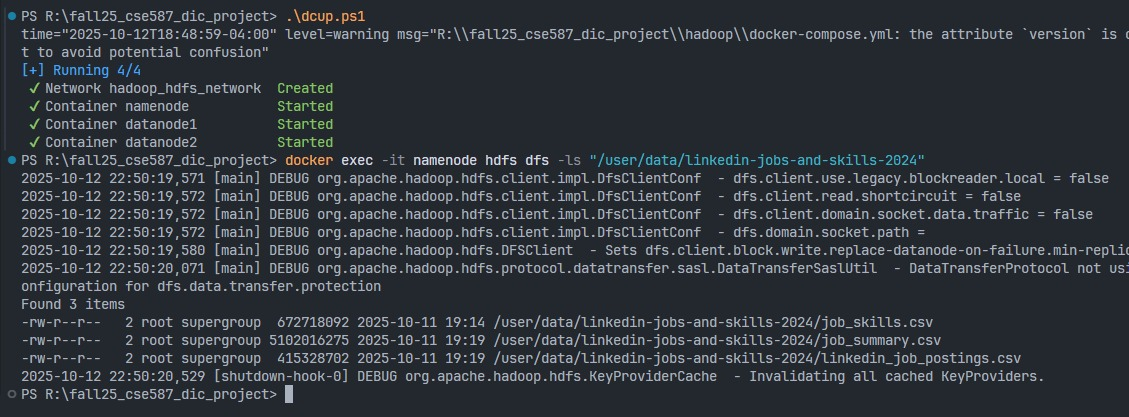
\includegraphics[width=\textwidth]{ih.jpeg}
    \caption{Hadoop cluster setup and Data Ingestion}
    \label{fig:placeholder}
\end{figure*}

Figure~\ref{fig:placeholder} For data ingestion, a PowerShell script was developed to automate the process of downloading and uploading a large Kaggle dataset, specifically \textit{asaniczka/1-3m-linkedin-jobs-and-skills-2024}, into the Hadoop Distributed File System (HDFS). The script first checked for the presence of the dataset locally; if not found, it used the Kaggle CLI to download and unzip the data into a temporary directory. Subsequently, it iterated through each CSV file in the downloaded dataset, performing a two-step transfer. First, it used \texttt{docker cp} to copy each file from the local machine into the NameNode container's temporary directory. Second, it executed the \texttt{hdfs dfs -put} command from within the container to move the files into the designated HDFS path, \texttt{/user/data/linkedin-jobs-and-skills-2024}. This methodical approach ensured a smooth and reliable transfer of all data. Final verification was performed by listing the contents of the HDFS directory with \texttt{hdfs dfs -ls}, confirming the successful ingestion of all files. The local temporary files were then cleaned up to conclude the process. This automated workflow streamlined the setup and data loading, providing a solid foundation for subsequent data processing and analysis tasks.

\section{\textbf{Results and Observations}}
The exploratory phase produced several meaningful insights about the global job market using LinkedIn’s 2024 dataset. The analysis combined frequency distributions, categorical summaries, and data visualizations to interpret hiring patterns across industries, job levels, and geographic regions. The following key observations were derived from the four main visualizations produced during EDA.

\subsection{Job Level Distribution}
Figure~\ref{fig:joblevel} illustrates the distribution of job levels across the dataset. The majority of postings belonged to mid-level and senior-level categories, indicating that companies are primarily hiring for roles that require prior experience. Entry-level and internship positions were less frequent, suggesting a competitive early-career environment. This pattern emphasizes the rising demand for experienced professionals in both technical and managerial domains.

\begin{figure}[htbp]
\centering
    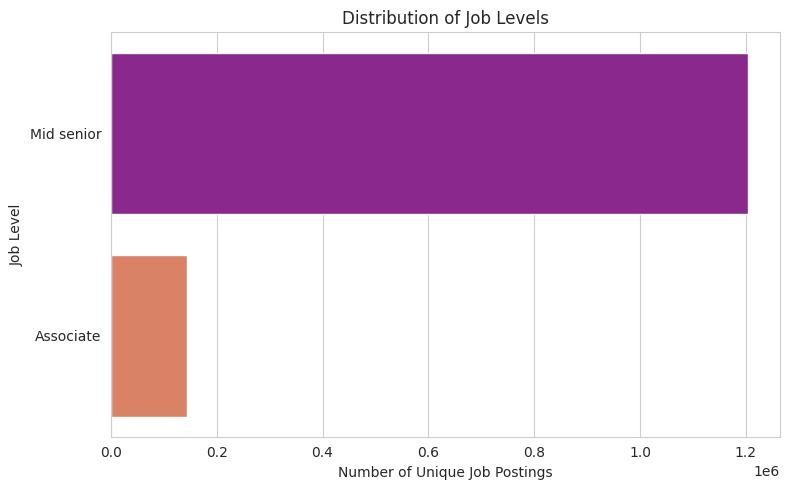
\includegraphics[width=\linewidth]{joblevels.jpeg}
\caption{Distribution of job levels across LinkedIn postings.}
\label{fig:joblevel}
\end{figure}


\subsection{Top Hiring Companies}
Figure~\ref{fig:companies} highlights the top companies contributing to the largest share of job postings. The visualization revealed that multinational technology and consulting firms dominated recruitment activity. Organizations such as Accenture, Amazon, IBM, and Deloitte consistently appeared among the most active recruiters, reflecting their global operational reach and diverse hiring needs. This trend aligns with the observed concentration of postings in technology-driven industries.

\begin{figure}[htbp]
 \centering
    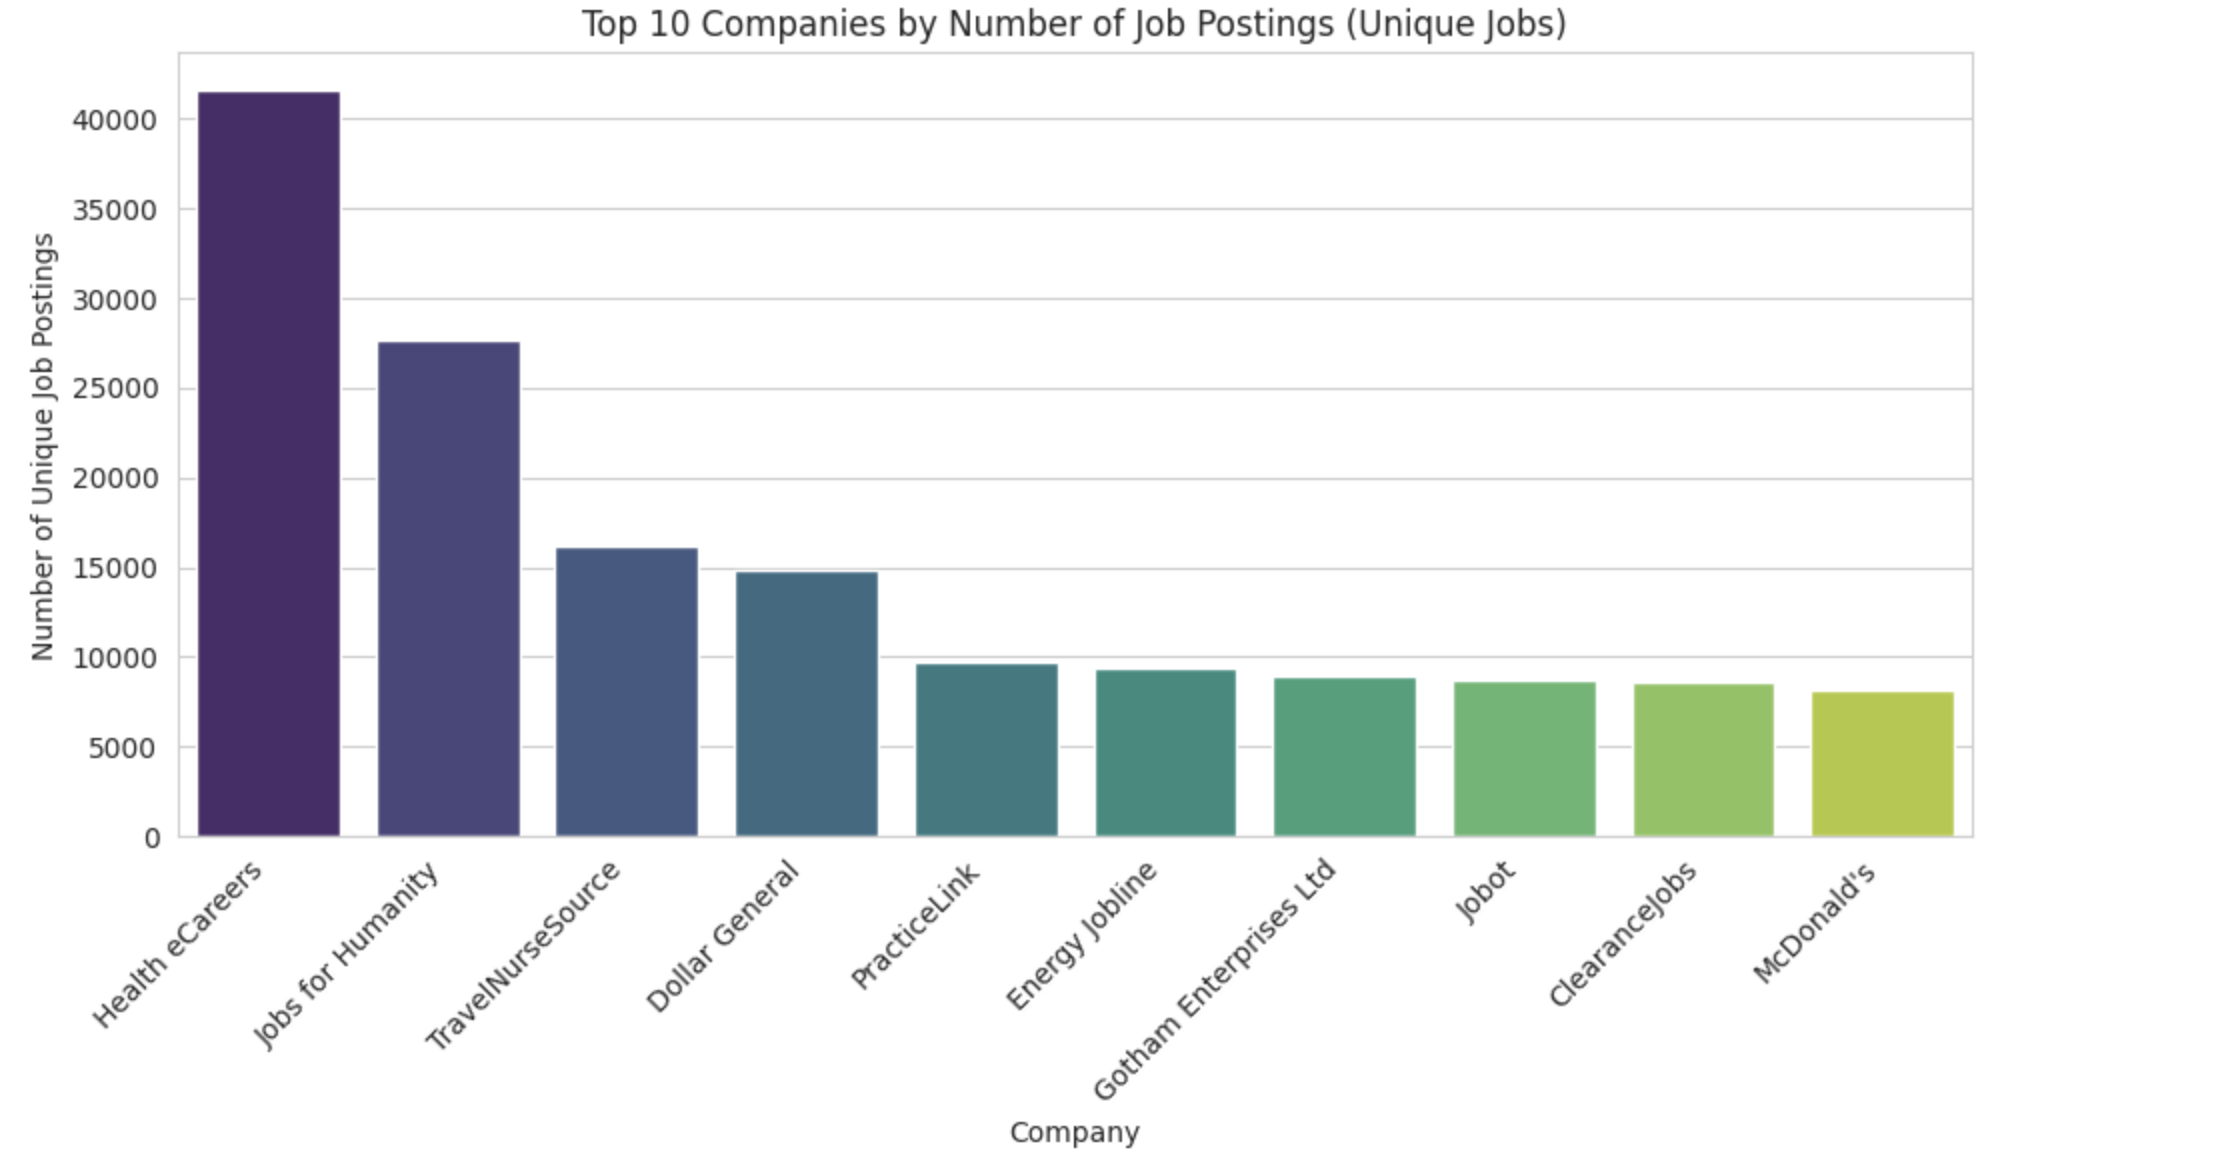
\includegraphics[width=\linewidth]{job_type_distribution.png}
    
\caption{Top companies by number of job postings.}
\label{fig:companies}
\end{figure}


\subsection{Job Type Analysis}
As shown in Figure~\ref{fig:jobtype}, full-time employment was overwhelmingly dominant, followed by remote, hybrid, and contract positions. This pattern underscores the continued preference for stable, long-term employment while also signaling the global adoption of flexible work models post-pandemic. The growing proportion of hybrid roles highlights a shift toward digitally adaptive workplaces.

\begin{figure}[htbp]
    \centering
    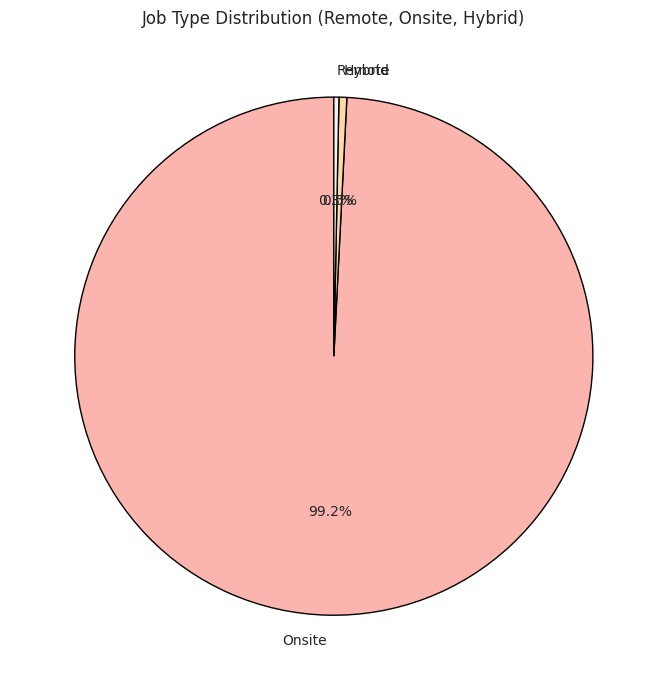
\includegraphics[width=\linewidth]{fig 1.jpeg}
    \caption{Distribution of job types (full-time, hybrid, remote, contract).}
\label{fig:jobtype}
\end{figure}


\subsection{Top Job Locations}
Figure~\ref{fig:locations} presents the top ten global cities with the highest job posting frequencies. New York, London, and Bangalore emerged as major employment hubs, followed by other metropolitan centers such as Toronto and Sydney. The distribution reflects economic centralization in key urban markets and a high concentration of opportunities in technology and finance sectors.

\begin{figure}[htbp]
    \centering
    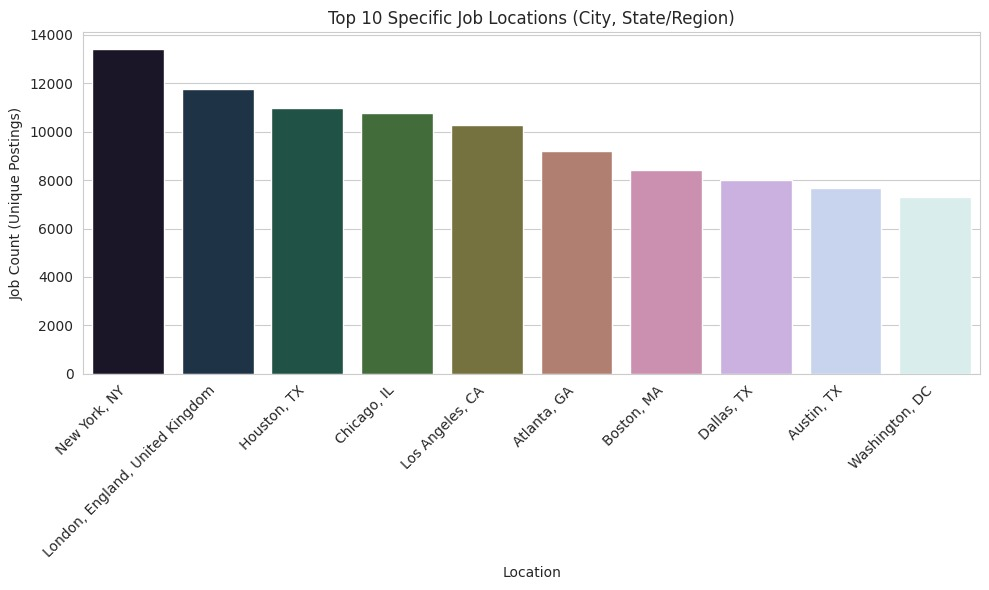
\includegraphics[width=\linewidth]{joblocations.jpeg}
\caption{Top global job locations based on posting frequency.}
\label{fig:locations}
\end{figure}


Overall, the visualizations provide a clear overview of employment patterns and labor demand dynamics across sectors and regions. The findings from this phase serve as a foundation for the next stage of analysis, which will focus on deeper skill correlation studies, clustering, and predictive modeling.



\section{\textbf{Conclusion and Future Work}}
This Phase 1 project successfully build a scalable big data framework to analyze the 1.3M LinkedIn Jobs and Skills (2024) dataset. The work in this phase revealed important global job market insights. Full-time roles were the dominant employment type, while hybrid and remote jobs continued to rise in prominence. Major hiring hubs included New York, London, and Bangalore, reflecting global economic centers. Job-level analysis showed a concentration of mid-level and senior positions, emphasizing demand for experienced professionals. Top hiring companies were primarily from technology and consulting sectors, and frequently required technical and analytical skills such as Python, SQL, Machine Learning, and Communication—demonstrating the growing blend of technical and soft skill demands across industries.  

Building upon these foundations, the next phase of this project will focus on achieving six analytical and machine learning objectives. These include: identifying global and regional skill trends, analyzing correlations between skills and job seniority, quantifying job similarity through skill overlap metrics, exploring regional specialization in skill sets, forming job clusters using unsupervised learning, and visualizing evolving skill categories across industries. Phase 2 will therefore shift from data preparation to advanced analytics, clustering, and predictive modeling, further leveraging the Hadoop ecosystem and machine learning tools.  

Overall, this phase demonstrated that LinkedIn’s large-scale job data can provide rich insights into employment structures and skill dynamics. The established data pipeline ensures scalability and reproducibility for subsequent analytical phases, laying a strong foundation for predictive and visual intelligence on global workforce trends.



\begin{thebibliography}{00}

\bibitem{linkedin}
A. Asaniczka, “1.3M LinkedIn Jobs and Skills (2024),” \textit{Kaggle Dataset}, 2024. [Online]. Available: \url{https://www.kaggle.com/datasets/asaniczka/1-3m-linkedin-jobs-and-skills-2024}

\bibitem{hadoop}
Apache Software Foundation, “Hadoop: Open-Source Distributed Computing Framework,” 2024. [Online]. Available: \url{https://hadoop.apache.org/}

\bibitem{pandas}
W. McKinney, \textit{Data Analysis with Pandas}. O’Reilly Media, 2022.



\end{thebibliography}

\end{document}
